The scenario of \textit{Open Set Domain Adaptation \textbf{(OSDA)}} constitutes a source domain ${D}_{s}=\{(x^i_s, y^i_s)\}_{i=1}^{n_s}$ of $n_s$ labeled samples and a target domain ${D}_{t}=\{x^j_t\}_{j=1}^{n_t}$ of ${n_t}$ unlabeled samples. 
The source samples are drawn from a label space $C_s$, which is shared by the target domain ${D}_t$, while the target domain is further associated with an additional label space $C_t/C_s$.
We define the classes from $C_s$ the \textbf{known classes} and classes from $C_t/C_s$ the \textbf{unknown classes} since we known nothing about them. 
Therefore, in the setting of OSDA, the label space of target domain contains the label space of source domain, \textit{i.e.}, $C_s \subset C_t$. 
The source and target domain are drawn from different probability distributions $p_s$ and $p_t$ respectively. 
In close set domain adaptation we have $p_s \neq p_t$; and in open set domain adaptation, we further demand the distributions of known classes are different, \textit{i.e.}, $p_s \neq p_{t_{C_s}}$, where $p_{t_{C_s}}$ denotes the distribution of the target samples belonging to label space $C_s$. 


\begin{figure}[!t]
    \centering 
    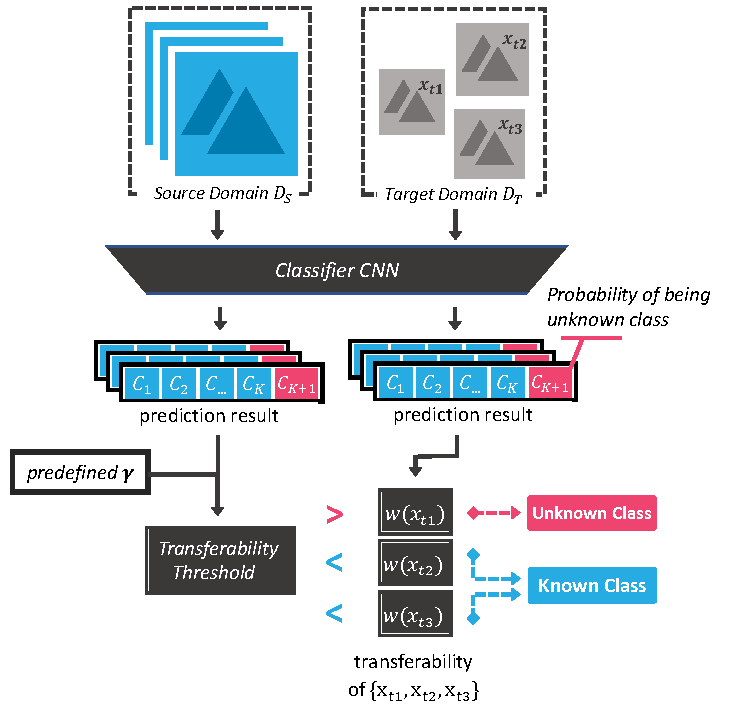
\includegraphics[width=0.48\textwidth]{contents/figures/pdf/selection.pdf} 
    \caption{
        The procedure of transferability based sample selection. 
        Given a batch of training samples, we calculate a transferability threshold by averaging transferability scores of source domain samples, and further tweak it during the training process.
        Then we select target samples whose transferability exceeds threshold as samples from the known classes, \textit{e.g.}, $x_{t2}$ and $x_{t3}$ are select for domain adversarial training. 
    } 
    \label{figure: selection} 
\end{figure}
\begin{figure*}
    \centering 
    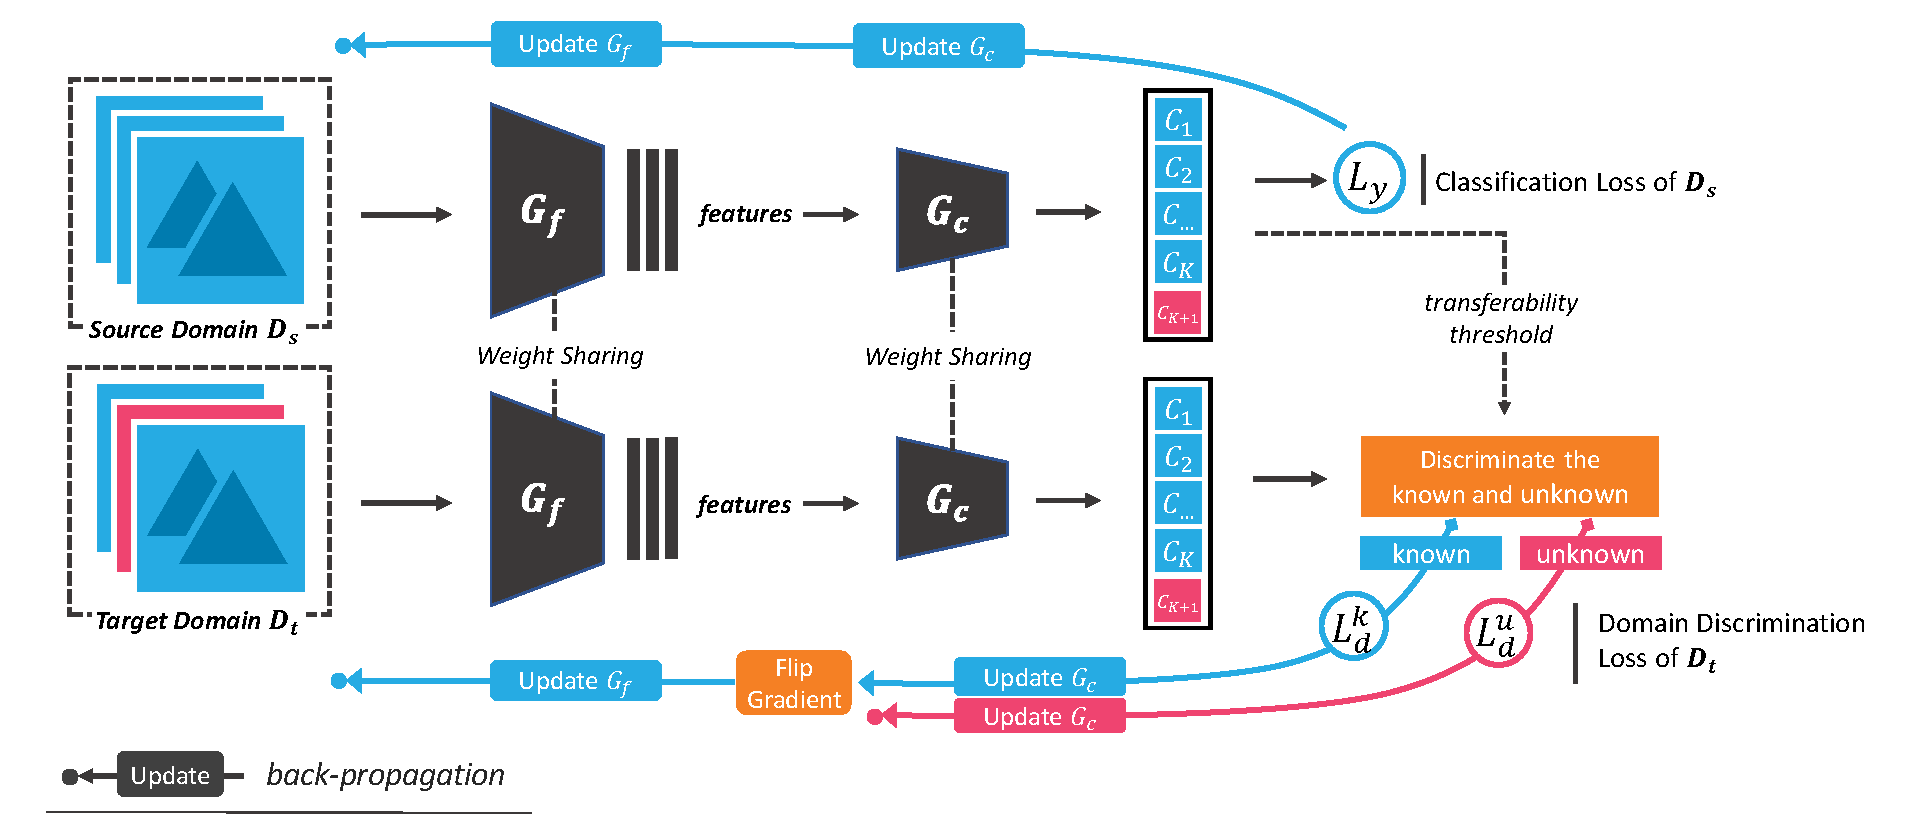
\includegraphics[width=0.95\textwidth]{contents/figures/pdf/ThDANN.pdf} 
    \caption{
        The network architecture of the proposed Thresholded Domain Adversarial Network \textit{\textbf{(ThDAN)}}. The classifier $G_C$ output $K+1$ dimensional probabilistic output after the $G_f$ extract features. For source samples, the $G_c$ and $G_f$ are trained to correctly classify them by minimizing classification loss $L_y$. For the target samples, we begin with splitting them into the known class partition and the unknown class partition according to \figurename{\ref{figure: selection}}, then calculate domain discriminate loss $L_d$ for this two partition respectivly. By minimizing $L_d$ to update $G_c$, we can correctly label the unknown class samples. In the aid of the gradient reversal layer (GRL), we can use $L_d$ to update $G_f$ to match the distribution between the known-marked samples and the samples of source domain.
    } 
    \label{figure: ThDANN} 
\end{figure*}

\subsection{Preliminary: Domain Adversarial Training}
\textit{Close Set Domain Adaptation \textbf{(CSDA)}} focuses on reducing the domain shift between the source and target domains.
Inspired by \textit{Generative Adversarial Network \textbf{(GAN)}} \cite{goodfellow2014generative}, Grain \textit{et al.} propose a \textit{Domain Adversarial Neural Network (\textbf{DANN})} \cite{DomainAdversrialNetwork} for CSDA by performing the domain adversarial training to align distributions between domains.
The domain adversarial training is a two-player minmax game: 
the domain discriminator $G_d$ as the first player aims to separate the feature representation of the source domain from the target domain, at the same time, feature generator $G_f$ as the second player is trained to deceive the domain discriminator. 
Formally, the domain adversarial training can be written as:
\begin{equation}
    \label{eq: training DANN}
    \begin{split}
        \min_{G_f} \max_{G_d} \mathscr{L}(G_f,G_d) &=\mathbb{E}_{x\sim p_t(x)} \left[ \log \left(G_d\left(G_f\left(x\right)\right)\right) \right]\\
        &+\mathbb{E}_{x\sim p_s(x)}\left[ \log \left(1-G_d\left(G_f\left(x\right)\right)\right) \right]
    \end{split}
\end{equation}
Since the feature extractor $G_f$ and domain discriminator $G_d$ are trained in adversarial manner, the $G_f$ and $G_d$ can be considered as the \textit{generative network} and \textit{discriminate network} of GAN respectively. 
Given any $G_f$ the optimal $G_d$ is:
\begin{equation}
    \label{eq: optimal discriminate}
    \begin{split}
        G_d^*(z) &= \frac{p_s(z)}{p_s(z)+p_t(z)}, \\
    \end{split}
\end{equation}
where $z$ is the features extracted by $G_f$, \textit{i.e}, $z=G_f(x)$.
We give the proof of Equation \ref{eq: optimal discriminate} as follows, 

\begin{proof}
    For any $G_f$, we train $G_d$ to maximize Equation \ref{eq: optimal discriminate}:
    \begin{equation}
        \label{eq: proof optimal discriminator}
        \begin{split}
            \max_{G_d} \mathscr{L}(G_f,G_d)  = &\int_x p_s(x)\log \left(G_d\left(G_f\left(x\right)\right)\right) 
            \\ & + p_t(x) \log\left(1-G_d\left(G_f\left(x\right)\right)\right) \, dx.
            \\ = &\int_x p_s(x)\log \left(G_d\left(z\right)\right) 
            \\ & + p_t(x) \log\left(1-G_d\left(z\right)\right) \, dx.
        \end{split}
    \end{equation}
    For any $(a,b) \in \mathbb{R}^2 \backslash \{0,0\}$, the function $y \to a\log(y) + b\log(1-y)$ achieves its maximum in $[0,1]$ at $\frac{a}{a+b}$.
    Therefore the optimal $G_d$ is Equation \ref{eq: optimal discriminate}.
\end{proof}


\subsection{Thresholded Domain Adversarial Network}
In the setting of OSDA, the target samples from the unknown classes are untransferable, since aligning distributions for them will incur the negative transfer. 
Based on this observation, this paper proposes a \textit{Thresholded Domain Adversarial Network (\textbf{ThDAN})} to tackle the challenge of OSDA by selecting transferable target samples for domain adversarial training.

In ThDAN, we construct a feature generator $G_f$ to extract domain-invariant features, and a classifier $G_c$ to correctly label samples from the common classes and reject samples from the unknown ones by leveraging features extracted by $G_f$. 
Following the practice of \cite{OpensetDA-bp}, we design the classifier $G_c$ as a $K+1$ ways network where $1\sim K$ dimensions indicate the probability for the known classes and the last dimension indicates the probability of being target samples. 
That means the last dimensional output of $G_c$ can be considered as a domain discriminator.
We use the superscript $k$ to denote $k'th$ dimensional output of $G_c^k$, then we naturally have $G_d=G_c^{K+1}$, which enables domain adversarial training for $G_d$.

We first train the classifier $G_c$ and the feature extractor $G_f$ to correctly categorize source samples $X_s$ through a standard cross-entropy loss $L_{ce}$:
\begin{equation}
    \label{eq: training ThDAN class}
    \begin{split}
        \min_{G_f,G_c} \mathscr{L}_s 
        &= \mathbb{E}_{(x,y) \in X_s} L_{ce}\left(G_c\left(G_f\left(x\right)\right), y\right).
    \end{split}
\end{equation}
To tackle the challenge of OSDA, we derive a sample selection algorithm based on transferability to divide a batch of target samples $X_t$ into the samples from the known classes and samples from the unknown classes, denoted as $X_t^k$ and $X_t^u$ respectively. 
Then we following the domain adversarial training to align distributions between the source samples and the target samples selected as samples from the known classes: 
\begin{equation}
    \label{eq: training ThDAN known}
    \begin{split}
        \min_{G_f} \max_{G_d} \mathscr{L}(G_f,G_d) &=\mathbb{E}_{x\in X_t^k} \left[ \log \left(G_d\left(G_f\left(x\right)\right)\right) \right]\\
        &+\mathbb{E}_{x \in X_s}\left[ \log \left(1-G_d\left(G_f\left(x\right)\right)\right) \right]
    \end{split}
\end{equation}
For the samples from $X_t^u$, we simply train $G_d$ to label them as target samples:
\begin{equation}
    \label{eq: ttraining ThDAN unknown}
    \begin{split}
        \max_{G_d} \mathscr{L}_u &=\mathbb{E}_{x\in X_t^u} \left[ \log \left(G_d\left(G_f\left(x\right)\right)\right) \right].
    \end{split}
\end{equation}
Since sample of $X_t^u$ are discarded during the domain adversarial training, the $G_d$ will confidently label them as the target data.
Therefore we can use the output of $G_d$ to approximate the probability of being the unknown class samples.
The architecture of ThDNA is illustrated in \figurename{\ref{figure: ThDANN}}.
In the following sections, we will introduce the sample selection algorithm in detail.

\subsection{Transferability Quantification}
Many works for domain adaptation \cite{PartialDA-iw,TransferableAttentionDA,PartialDA-tf} utilize the concept of transferability as an attention mechanism to reweight the importance of samples, so that the model can pay more attention to the transferable samples and inhibit the negative transfer caused by the untransferable ones. 
In the seething of OSDA, the samples from the known classes should be more transferable than the target samples from the unknown classes.
Based on this observation, we derive a criterion to quantify the transferability to select transferable target samples for domain adversarial training.

\textbf{Target samples from the known classes are able to confuse $G_d$.}
Considering the network $G_d$ has converged to the optimal value for the current feature extractor, the output value of it delivers the likelihood of the sample from the target domain. 
For a target sample, if $G_d^*(z)$ approaches to $1$, then the sample has a high probability of coming from the unknown classes.
That is because the unknown classes only included in the target domain and can be almost perfectly discriminated from the source samples. 
On the other hand, if $G_d^*(z)$ approaches to $0$, then the sample is more likely from the known classes that shared by domains. 
Therefore, the transferable target samples are able to confuse $G_d$ to label them as the source samples.
Then we define the transferability $w_d(x)$ as inversely related to $G_d^*(z)$ that given in Equation \ref{eq: optimal discriminate}:
\begin{equation}
    \label{eq: domain transferability}
    \begin{split}
        w_d(x) = 1-G_d^*(z)=  1-\frac{1}{1+p_t(z)/p_s(z)}.\\ 
    \end{split}
\end{equation}
Equation \ref{eq: domain transferability} indicates the labeled samples from the source domain should be more transferable than unlabeled ones from the target domain. 
Note that the weights function is also a function of density ratio between target and source features.
This further verifies the reasonableness of the weights function, since target samples from the known classes will give a higher value of $p_s(z)$ due to the overlapping of marginal distribution with source samples. 


\textbf{Target samples from the known classes can be categorized by $G_c$.}
We use the superscript $k$ to denote $k'th$ dimensional output of $G_c^k$, then the probability distributions among the known classes are: 
\begin{equation}
    \label{eq: softmaxed}
    \begin{split}
        G_{c,\; known}=softmax([G_c^1,G_c^2,...,G_c^K]).
    \end{split}
\end{equation} 
Due to the overlapping in the marginal distributions, the target samples from the known classes should be categorized by the classifier $G_c$ that trained on the source samples.
As the \textit{entropy} measures the degree to which the probability of the model is spread out over different possible states, it can be used to measure the uncertainty of predictions. 
Therefore we can utilize the entropy to measure if a target sample can be categorized by $G_c$.
Then we define the transferability $w_c(x)$ as inversely related to the classification entropy: 
\begin{equation}
    \label{eq: class transferability}
    \begin{split}
        w_c(x)&=1-H(G_{c,\; known}(z)).
    \end{split}
\end{equation}
where the $H(\cdot)$ is the \textit{normalized entropy} whose value between $0$ and $1$. 
Since the classifier is trained by the supervised information from the source domain, it will make a solid prediction for source samples and deliver low entropies, so the source samples should be more transferable then the target samples. 
And for samples from the unknown classes, because they cannot be aligned with a specific class from the source domain, the prediction tends to be uncertain over $K$ known categories, which leads to the high prediction entropy and low transferability. 

Since the domain discriminate $G_d$ in Equation\ref{eq: domain transferability} and the classifier $G_{c, known}$ in Equation\ref{eq: class transferability} work independently, we can unify the transferability as,
\begin{equation}
    \label{eq: transferability}
    w(x)=1-G_d(z)\cdot H(G_{c,\; known}(z)).
\end{equation} 
As stated before, the source samples should be most transferable, and the target samples from the known classes should be more transferable than ones from the unknown classes. 
Ideally, the transferability holds the following inequality, 
\begin{equation}
    \label{eq: inequation of transferability}
    \mathbb{E}_{x \sim p_s}w(x)>
    \mathbb{E}_{x \sim p_{t_{C_s}}}w(x)>
    \mathbb{E}_{x \sim p_{t_{C_t/C_s}}}w(x).
\end{equation}



\subsection{Transferable Sample Selection}
In this section, we present the sample selection algorithm to select transferable target samples for domain adversarial training based on transferability criterion in Equation\ref{eq: inequation of transferability}. 

We begin by adaptively computing a \textit{transferability threshold} $\beta$ as follows, 
\begin{equation}
    \label{eq: transferability thresholded}
    \beta(X_s, \gamma_0) = \mathbb{E}_{x \in X_s} w(x) - \gamma_0.
\end{equation}
The threshold is calculated by averaging the transferability score of a batch source samples $X_s$ and a predefined constant $\gamma_0$. 
Note that the $\gamma_0$ is used for adjusting the threshold so as to control the acceptable range of target samples, \textit{i.e.}, lowing the value of $\gamma_0$, we can gather a smaller batch of more transferable samples, on the other hand, raising the value of $\gamma_0$, we can gather a bigger batch of less transferable samples. 

Then, as is shown in \figurename{\ref{figure: selection}, the target samples whose transferability score exceeds the threshold $\beta$ are selected as the samples of known classes, and others as the samples of unknown ones. 
In particular, for a batch of target samples $X_t$, we divide it into two partitions based on the transferability threshold $\beta$: 
\begin{equation}
    \label{eq: split target examples}
    \begin{split}
        X_t^k=\{x|w(x) \geq \beta, x \in X_t \}, \\
        X_t^u=\{x|w(x) < \beta, x \in X_t \}.
    \end{split}
\end{equation}
Here $X_t^k$ and $X_t^u$ are target samples selected as the known classes and unknown classes respectively.
For samples of $X_t^k$, we adopt the domain adversarial training to align distributions with source samples as Equation\ref{eq: training ThDAN known}.
For samples of $X_t^u$, we train the domain discriminate $G_d$ to label them as samples from the target domain as Equation\ref{eq: ttraining ThDAN unknown}.

\subsection{Progressive Sample Selection}
\label{Section : Progressive Sample Selection}
Sample selection is the key step for ThDAN to tackle the challenge of OSDA. 
However, due to the limited computing resources and the changeability of transferability, the selection algorithm based on Equation \ref{eq: transferability thresholded} may not convey the best result. 
In order to improve the accuracy of sample selection, and select more target samples from the known classes for training, this section proposes a \textit{Progressive Sample Selection} strategy by progressively tweaking the transferability threshold during training process. 

By the reason of limited computing resource, most deep learning models can only be trained in the stochastic way. that is, our model receives a mini-batch of training samples $X_S$ and yields a \textit{stochastic} transferability threshold based on Equation\ref{eq: transferability thresholded}. 
Since the threshold is calculated by averaging the transferability score of source samples, the mini-batch training may lead to the oscillation of threshold, and further decay the accuracy of sample selection. 
To alleviate oscillation of transferability threshold, this paper refers to \cite{MomentumSGD} and introduces the idea of \textit{momentum}. 
Instead of using only the threshold of the current step to guide the selection, the momentum also accumulates the threshold of the past steps to reduce the randomness of mini-batch training.  
Using $\beta^*$ to denote \textit{momentum transferability threshold}.
For the first mini-batch training samples $X_{s_0}$, we simply follow Equation\ref{eq: transferability thresholded} to calculate $\beta^*$, 
\begin{equation}
    \label{eq: momentum transferability baseline}
    \begin{split}
        \beta_n &= \beta(X_{s_n},\gamma), \\
        \beta^*_0 &= \beta_0.
    \end{split}
\end{equation}
For the $n'th$ mini-batch training samples $X_{s_n}$, the $\beta^*$ is computed with momentum,
\begin{equation}
    \label{eq: momentum transferability baseline}
    \begin{split}
        \beta^*_n &= m \cdot \beta_n + (1-m) \cdot \beta^*_{n-1} .
    \end{split}
\end{equation}
where $m$ is the momentum scalar lies in $(0,1]$. The momentum threshold is a weight sum of current value and previous value. 
By introducing the idea of momentum, the oscillation of the transferability threshold can be alleviated.

Besides the oscillation of mini-batch training, the sample selection algorithm also suffers from the continuous change of transferability of samples. 
In particular, since the model are trained to correctly label target samples from known classes and reject the samples from unknown ones, the transferability of the former will gradually increase, whereas the transferability of the latter will gradually decrease. 
Therefore, using a fixed $\gamma$ to calculate the transferability threshold may not be a good choice. 
To maximize the accuracy of the sample selection, $\gamma$ should be small at an early stage so that the model can select the target samples that are most likely to be the known classes. 
As the training goes, the $\gamma$ progressively increases, so that more target samples from the known classes can be correctly selected for training. 
To facilitate sample selection, this work progressively increases the value of $\gamma$ by a piecewise function based on training step $n$:
\begin{equation}  
    \label{eq: dynamic tolerable range}
    \begin{split}
        \gamma(n) &= 
        \begin{cases}
            0 & ,\: n \in N_1 \\
            \gamma_0 \times  \sigma(n) & ,\: n\in N_2 \\ 
        \end{cases}
    \end{split}
\end{equation}
where $N_1$ is the steps where we set $\gamma$ to $0$, and $N2$ is the steps where we progressively increase $\gamma$ based on a \textit{monotonically increasing function} $\sigma(\cdot)$ with an upper bound of $1$. 
Initially, by setting $\gamma$ to $0$, the target samples that are more transferable than the source samples are selected as samples of known classes, thus maximizing the accuracy of the sample selection. 
After the model has aligned with these samples, the $\gamma$ will progressively increase so as to collect more samples to enhance domain adversarial training. 

% \subsection{Training Procedure}
% This paper introduces a model namely \textit{Thresholded Domain Adversarial Network (\textbf{ThDAN})}, which tackles the challenge of OSDA by domain adversarial training with sample selection. 
% We begin by demonstrating the training procedure of the ThDAN. 
% Initially, we train the classifier $G_c$ and the feature extractor $G_f$ to correctly categorize source samples $X_s$ through a standard cross-entropy loss $L_{ce}$:
% \begin{equation}
%     \label{eq: source classification loss}
%     \begin{split}
%         L_y
%         &= \mathbb{E}_{(x,y) \in X_s} L_{ce}(G_c(G_f(x)), y)
%     \end{split}
% \end{equation}


% Using $G_d$ to denote last dimension output of $G_c$, \textit{i.e.}, $G_d=G_c^{K+1}$. For target samples $X_t$, we divide it into a partition of known class $X_t^k$ and a partition of unknown class $X_t^u$ according to Equation\ref{eq: split target examples}. Then we train the $G_d$ to discriminate the target samples from the unknown class partition $X_t^u$ by minimizing a binary-cross-entropy loss $L_{bce}$: 
% \begin{align}
%     \label{eq: domain adversarial classify}
%     L_d^u = \mathbb{E}_{x \in X_t^u}L_{bce}(G_d(G_f(x)), 1).
% \end{align} 
% Note that we do not explicitly train $G_d$ to discriminate source samples, that is because Equation\ref{eq: source classification loss} ensures $G_d(G_f(x_s))=0$. 

% In order to generated domain-invariant features, we follow the domain adversarial training proposed in \cite{DomainAdversrialNetwork}. First, we train $G_d$ to discriminate the samples from $X_t^k$,
% \begin{align}
%     \label{eq: domain adversarial classify known}
%     L_d^k = \mathbb{E}_{x \in X_t^k}L_{bce}(G_d(G_f(x)), 1).
% \end{align} 
% Then we train the feature extractor $G_f$ to deceive the discriminator $G_d$ with the help of \textit{gradient reversal layer}. 
% The gradient reversal makes it possible to flip the sign of the gradient during the backward propagation, which enables end-to-end training of the ThDAN. 
% Using $\theta_f$, $\theta_d$ and $\theta_c$ to denote the parameters of $G_f$, $G_d$ and $G_c$ respectively, then the final objective of the proposed ThDAN is delivering the optimal $(\hat{\theta_f}, \hat{\theta_c}, \hat{\theta_d})$ by :
% \begin{align}
%     (\hat{\theta_f}, \hat{\theta_c}) 
%     &=  \arg  \; \underset{\theta_f, \theta_c}{\min} \;L_y - L_d^k, 
%     \label{eq: saddel of domain adversarial for d} \\ 
%     \hat{\theta_d} 
%     &= 
%     \arg  \; \underset{\theta_d}{\min} \;L_d^k+L_d^u. 
%     \label{eq: saddel of domain adversarial for f c}
% \end{align}
% Note that the model only aligns distribution between the source samples and the selected samples in $X_t^k$. As for the samples in $X_t^u$, it will be rejected as unknown classes, which means when the classifier $G_d$ trained to label them as an unknown class, the feature extractor $G_f$ will not try to confuse it. 
The detailed training procedure of ThDAN is presented in Algorithm1. 
\makeatletter
\newcommand{\removelatexerror}{\let\@latex@error\@gobble}
\makeatother

\begin{figure}[!t]
    \removelatexerror
    \begin{algorithm}[H]
    \caption{Learning algorithm for ThDAN}
    \KwData{
        \\the source datasets $\{(x^i_s, y^i_s)\}_{i=1}^{n_s}$ ; 
        \\the target datasets $\{(x^i_t)\}_{i=1}^{n_t}$.
    }
    \BlankLine 
    \KwIn{
        \\the $N_0$, $N_1$ and $N_2$ for dynamic training; 
        \\the upper bound $\gamma_0$ of tolerable range; 
        \\the trainable network $(G_f, G_c)$.
    }
    \BlankLine 
    \KwOut{
        \\an optimal solution $(\hat{G_f}, \hat{G_c})$.
    }
    \BlankLine 
    initialization\;
    \While{not converged}{
        Sample mini-batch $X_s$ from $\{(x_i^s, y_i^s)\}_{i=1}^{n_s}$\;
        Sample mini-batch $X_t$ from $\{(x_i^t)\}_{i=1}^{n_t}$\;
        \eIf{in pretraining staget $N_0$}{
            Update $G_f$, $G_c$ by (\ref{eq: training ThDAN class})\;
        }
        {
            Calculate the $\gamma$ by (\ref{eq: dynamic tolerable range})\;
            Calculate the \textit{transferability threshold} $\beta$ by (\ref{eq: momentum transferability baseline})\;
            Gather mini-batch of $X_t^k$ and $X_t^u$ from $X_t$ by (\ref{eq: split target examples})\;
            Update $G_f$, $G_c$ by (\ref{eq: training ThDAN class})\;
            Update $G_f$, $G_c$ by (\ref{eq: training ThDAN known}, \ref{eq: ttraining ThDAN unknown})\;
        }
    }
    \Return{
        $(\hat{G_f}, \hat{G_c}) = (G_f, G_c)$
    }  
    \end{algorithm}

\end{figure}



